\section{Design Landscape}
The purpose of designing a crypto-asset backed stablecoin is to create a stable asset out of a volatile asset. There are a number of stablecoins using crypto-assets as collateral to issue stablecoins which shows a very broad design landscape for indirectly-backed stable coins.

In this part, we propose a systematical design-decision model for indirectly-backed stablecoins. There are some key design decisions for each core feature. We describe core features and the key design decisions related to the main features, and also we will discuss the pros and cons of each feature.

An overview of the indirectly-backed stablecoins design landscape is in Figure \ref{land}.

\begin{figure*} [ht]
\centering
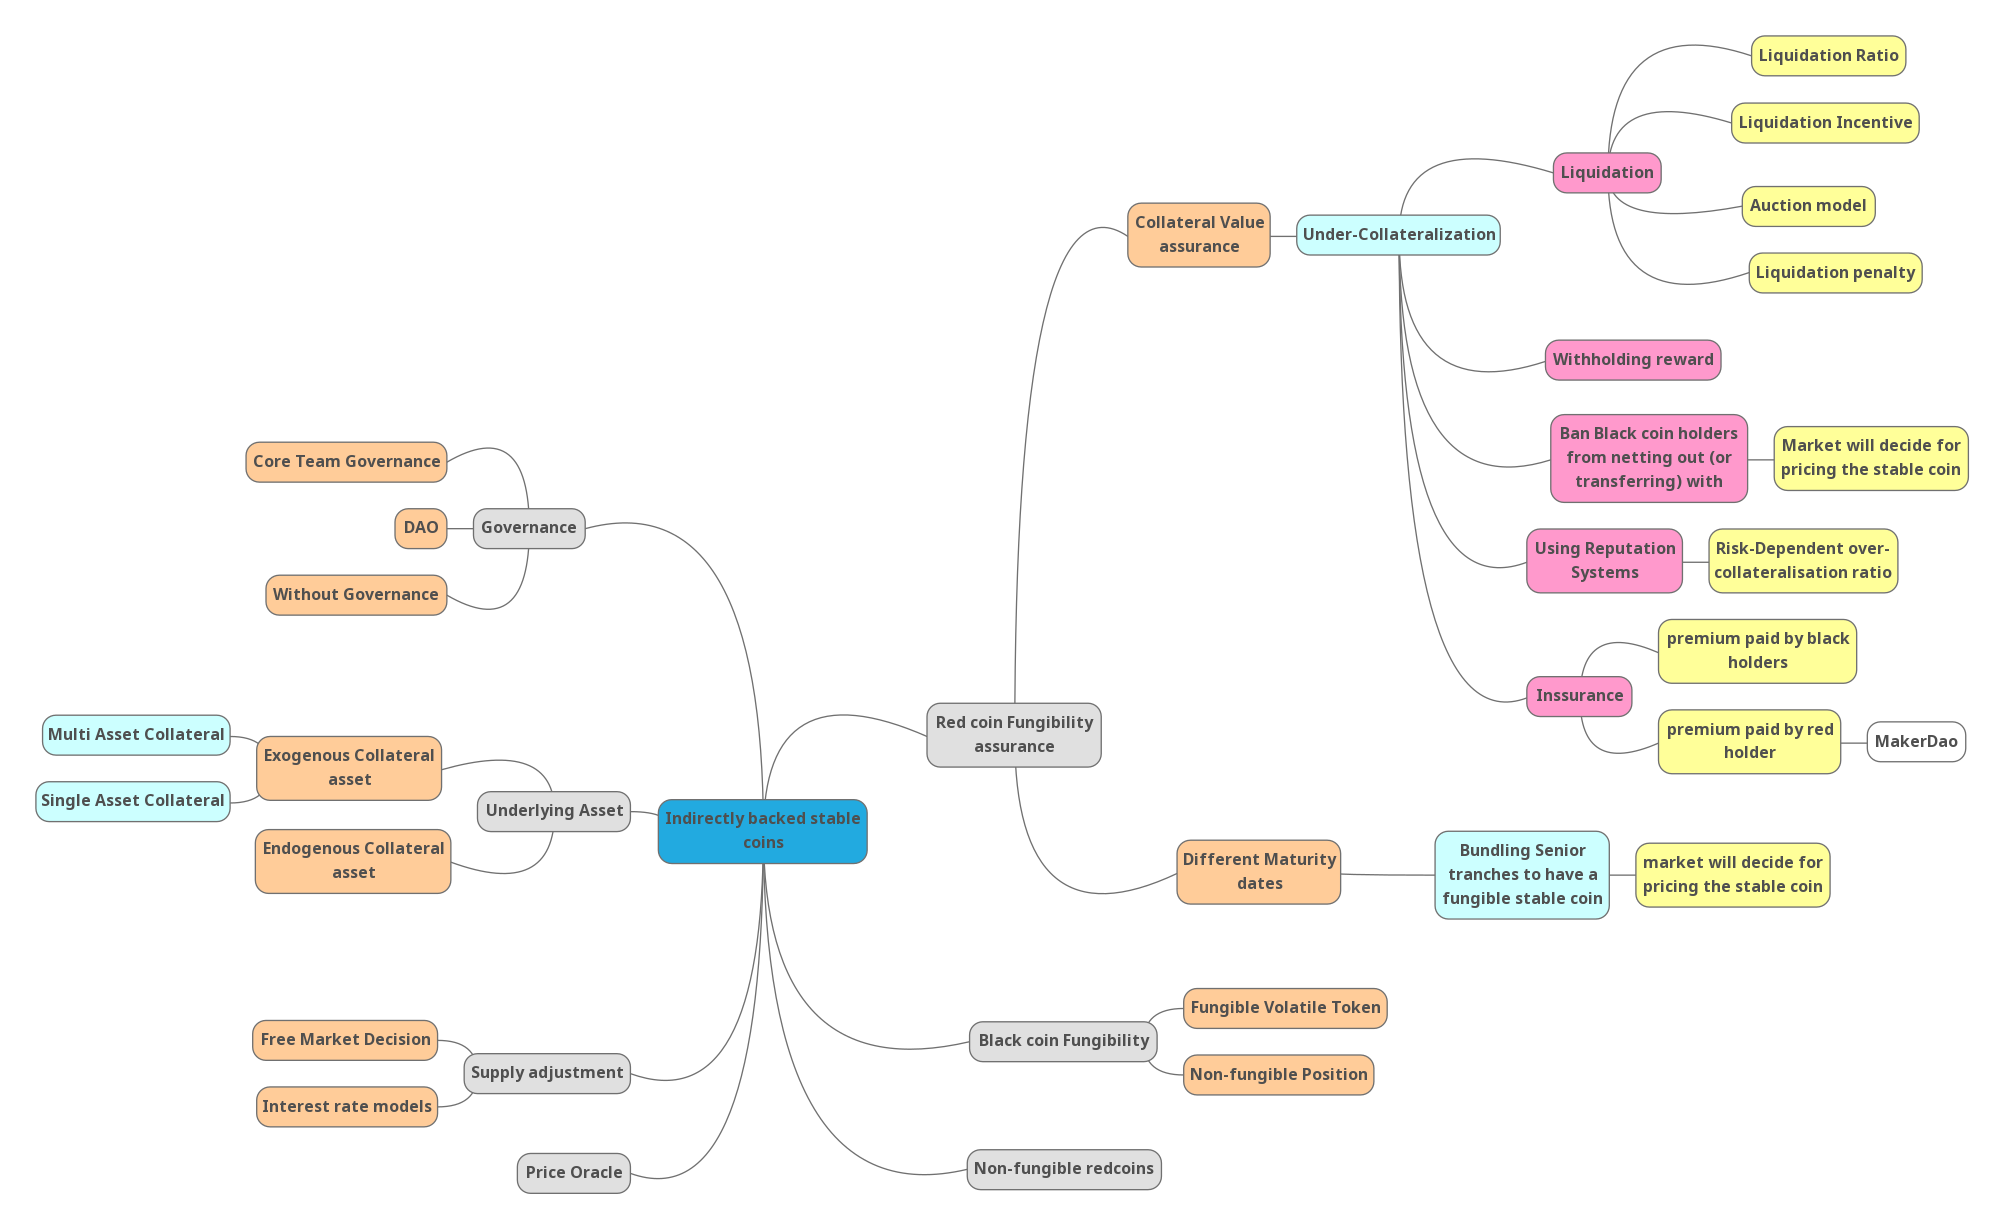
\includegraphics[width=16cm]{Mindmap}
\caption{overview of the indirectly-backed stablecoins design landscape}
\label{land}
\end{figure*}

\section{Fungibility}
Fungibility or Interchangeability refers to the feature of an asset to be exchanged by the same asset type with equal quality and quantity. For instance, dollar bills are fungible because people can exchange the same amount of dollars without any frictions.

The first design decision is whether the tokens on the systems should be fungible or should be non-fungible. 

Fungiblity decision is devided into two parts:
\begin{itemize}
  \item Red coins Fungibility
  \item Black coins Fungibility
\end{itemize} 
We will discuss them seperately on next sections.


\subsection{Red coins Fungibility}
The Red coins, the stable coin of the system, could be fungible or non-fungible. All currently implemented indirectly-backed stablecoins are using fungible stablecoin design. However, it could be non-fungible as well.

\subsubsection{Non-fungible Red coins}
A stablecoin system designer could allow red coins to be non-fungible. For instance, each token could be backed by a different amount of ETHs without limitations on the system such as collateral ratio, liquidation and etc.

In this design class, the Red coin and Black coin should be pair-wise. Because each pair is backing by a different vault and a specific amount of deposited ETH.

There should be a system parameter for each red coin, depends on its vault to distinct the coins.
For example, each red coin could be marked by debt to collateral ratio, the number of minted red coins divided by the value of deposited ETH on the related vault, which clarifies the safeties of the coin.
So the buyer could have speculation on the price of each red coin base on the debt to collateral ratio.

Some reasons push designers to make red coins fungible. The first reason is usability. Assume that Alice wants to buy 100 red coins. On the other side, Bob wants to sell just 30 coins, Carol wants to sell 50 and David wants to sell 20 red coins. Now Alice should make a price speculation of three different coins and buy them at different prices which is not convenient for her.

The other issue with the non-fungible red coins is price discovery. Markets and crowd wisdom help to aggregate different opinions on the value of an asset. The aggregated results will discover the efficient price of the asset. In non-fungible design, there is not a straight relation between the price of each red coin and the specific characteristic of them like the debt to collateral ratio. So, Each person has speculation for each coin. Because of non-fungibility, the aggregations would not happen and so the real price will not be discovered.

The other reason is that stable coin users are willing to use the stable coins as a money. So, they need stable coins serve as a unit of account which means that you can price other goods or assets using the stable coin. In non-fungible design each red coin has a specific price. So, users can not price other goods based on the stable coin.


\subsection{Fungible Red coins}
As mentioned in the previous part, stable coin designers put all their effort to create stable coin systems including fungible red coins. There are different mechanisms to bring fungibility into red coins. We classify them into two key designs discussed in the next sections.

\begin{itemize}
  \item Under-collaterallization
  \item Separate maturity dates
\end{itemize} 


\subsubsection{Collateral Value Assurance}

One of the methods to bring fungibility into red coins is to set a lower limit for vaults (Collateralization ratio). If the value of deposited ETH in a vault drops beneath a specific amount, then the system decides to take an action. 

In this circumstance, there is a minimum amount of ETHs (collateral ratio)  backing each red coin. It secures the fungibility of red coins. Red coin holders are sure that there is at least a dollar in the vault for their red coin  (strongly expected). There is no difference between their red coin and the red coin of other people in this circumstance.

We will discuss various designs that differ on how they secure the vaults from the under-collateralization in the next sections. Some of them are incentivizing vault keepers to keep their deposit more than collateralization ratio and some of them are disincentivizing the bad actors of the system.
 
\paragraph{Liquidation}
This variety of design is similar to the marginal accounts in traditional finance. If the underlying asset decreases in price and the value of a vault runs under the collateralization ratio, the system will liquidate the vault.

Liquidation occurs in the case that a vault is the danger area and may not able to pay its obligation. The deposited assets will transfer to the person who takes the responsibility of the debt of the vault. In other words, the liquidator should pay the borrowed red coin (and other obligations in a type of design, such as stability fee in MakerDAO) and receive the vault in exchange.


In liquidation design, the majority of vaults are over-collateralized. If a vault goes under-collateralize it will be liquidated. So, the red coin holders are pretty sure that their coin is backed by a dollar (. They can exchange their asset because the red coins are similar.

Smart contracts cannot trigger themselves. So, there should be an outsider player (like Keepers in MakerDao) to liquidate the warned vaults. They should trace the system to find the under-collateralized vaults and call the liquidation function. Then the keeper will transfer the debt of the vault to the smart contract and receive the deposit of the vault in exchange.

There are design parameters in the liquidation method:

\begin{enumerate}
  \item Collateralization Ratio:
This number shows the factor of over-collateralization. The ratio between the value of the deposits on each vault and the value of borrowed red coins should always be more than the collateralization ratio.
  
The collateralization ratio is depending on the volatility of the underlying asset. For instance, in the MakerDAO platform, the collateralization ratio for ETH vaults is 1.5. However, in the Synthetix project, it is 7.5 for SNX token, which is more volatile than ETH.
  \item Liquidation Incentive:
A smart contract is not able to trigger itself. An outsider player named liquidator should pay the transaction fee to call the liquidation function of the smart contract. Some factors influence the costs and profit of liquidators:
\begin{enumerate}
	\item Transaction fee:
The liquidator should trigger the liquidation function, send the sufficient red coins, and bid on the auction to win the vault. The user has to pay the transaction fee for these processes. The transaction fee depends on the time of transaction and network congestion.  
	\item Cost of capital: The liquidator pays the obligation by Red coin and receives the deposited coins of the vault. Therefore, the liquidator needs a sufficient amount of red coins for liquidation. There is an opportunity cost associated with the decision of the liquidator to not lend her capital and gain interest.

In other scenarios, the liquidator may just borrow the fund from lending platforms to liquidate the vault and pay back the loan afterward. There is a cost of borrowing in this scenario as well. So, there is a cost of capital for the liquidator.
	\item Price Oracles: RB coin systems need the price of the underlying asset in USD. Blockchains have no access to externals data. Oracles are outsider systems that collect the price and push them to the blockchains. Price inefficiency may impose extra costs on the liquidator. For instance, if the price of the asset is \$100 on the markets, although the oracle price is \$90, the liquidator spends more to provide liquidity from the markets.
\end{enumerate}  

The designer has to incentivize the liquidators to trace the blockchain, find alerted positions, and then send transactions to liquidate them. 

The mechanism of the incentivization is varied between protocols. A majority of platforms give the liquidator discounts on the vaults. For instance, in Single Collateral DAI (SAI), there was a \%3 discount on the liquidation process. Other platforms are using auction models to let the market decide about the value of the vault. 
  
  \item Auction model:
In the case of liquidations,  liquidators may come up with a specific warned position and want to liquidate it. The system designer has different options for the decision of picking the winner liquidator.
 
The simplest implementation mechanism is the First Come First Serve. However, it won't be fair for the vault holder if the first liquidator bids with a low amount of red coins.

There are other auction-based mechanisms to find the liquidator. The question raised here is, which method is the most efficient and fair auction model for both bidders and vault holders.

MakerDao utilizes a mixture of an absolute-auction and a reverse-auction model for the liquidation process.

The absolute auction model is used until the bids cover the debt of the vault. When the bids pass the debt, the auction reversed, the bidders bid on a lower amount of the deposits on the vault for a specific amount of DAI tokens, specified on the absolute auction step.
  
  \item Liquidation penalty:
The liquidation penalty is an extra punishment for the black coin holders to care about their debt to collateral ratio.
MakerDAO platform charges liquidated vault extra \%13 as a punishment for their vault holders. There are two main reasons to add Liquidation penalty on the design:

\begin{enumerate}

  \item To force vault keepers to be over-collateralized
  \item To mitigate grinding attacks: grinding attack occurs when the position holder deliberately unsafe her black coin and participate in the liquidation auction against her position to buy her deposited assets cheaper.

\end{enumerate}
\end{enumerate}

Using liquidation mechanism as a shield to protect the system provoke criticism. Possibly the black coin holders are freaking out when the price of ETH drops significantly. They may proceed to net out just before the liquidation occurs to their vaults. We called this situation "early liquidation" of the system. 

In this case, the system needs more ETHs to be deposited. The liquidation mechanism is designed to force the black coin holders to inject more ETHs to the system, but the black coin holders withdraw their deposits, and the total collateral of the system drops significantly, which is not the goal of the designers in this situation.

\paragraph{Withholding rewards}

Majority types of designs like liquidation are disincentivizing bad actors. But, another approach is to encourage users to act properly and incentivizing good actors of the system.

For instance, in the Synthetix project users need collateralize SNX tokens (Synthetix network token) to receive sUSD tokens (Synthetix stable coin pegging a USD). There is no margin call methods or liquidation function on the design. But, there is a reward on the system for users who keep more than the over-collateralization ratio. 
The Synthetix system has \%2 annual inflation on SNX tokens. The inflationary tokens are allocated to the vaults that hold more than the collateralization ratio.

There is another reward for the system. The traders on the exchange of the Synthetix project, pay transfer fees collected and distributed to the vaults holding more than the collateral ratio.

The system incentivizes people to stake their SNX token to be over-collateralized and receive the rewards. So, there is no punishment in the system for bad actors in this class of design.

\paragraph{Banning Black coin holders}

In the design of indirectly-backed stable coins, the red coins are not redeemable. In other words, the red coin holders cannot give back their red coins to receive \$1 of the deposited ETH in exchange. The red coin holder must own (or buy if possible) a black coin to net out a vault and receive the ETH.

In the liquidation scenario, the designer pushes black coin holders to be over-collateralized, applying liquidation punishments. Red coin holders and arbitragers are confident that there is no difference between the red coins because each of the red coins is backed by a sufficient amount of ETHs to be \$1 (with high probability).

In another class, the designer removes the liquidation mechanism, prevent black coin holders from withdrawal. In the fungible black coin design class, the designer also forbids the black coin holders from transferring their token. 

In this situation, the incentives for black coin holders to be over-collateralized has been decreased, compared to liquidation design class. But, there is a huge incentive left for them to be over-collateralized. If the price of the underlying asset drops, the black coin holders may want to sell their deposited assets to reduce the loss. In this scenario, just black coin holders that have over-collateralized vaults can net out and receive their underlying assets to sell them to the market.

This type of design will increase the fluctuation of the price of the red coin. The market watches the aggregated collaterals on the system and the number of red coins issued by the system and also the price of the underlying asset to evaluate the price of red coins. So when the price of underlying asset drops, the price of red coins will reduce concerning the underlying asset price. 

In this scenario, red coin holders are taking parts of the risk of underlying asset volatility risk. On the situation that the price of the asset drops significantly, the value of the stable coin will fall.

\paragraph{Reputation systems}

In traditional finance, reputation scoring systems are used to decrease or eliminate the collateral needs for a specific financial transaction. Participants are utilizing their reputation as collateral or source of trust for financial services. 

For instance, in the FICO credit score system, users can enhance their credit limit by increasing their credit score. There is a default risk on credit systems, but the defaulted person will be punished by credit score reduction. The bad actor loses reputation scores forbidden from using plenty of financial services. Therefore, users have adequate incentives to pay their bills.

A revolution of decentralizing the finance products on top of blockchain technologies began in early 2018, named Decentralized Finance (Defi) movement. There is a myriad of different decentralized financial services out there, such as MakerDAO, Compound, Synthetix, Aave, etc. 

There are no differences between users that act properly on Defi platforms and the bad actors. The DeFi ecosystem suffers from a lack of a reputation system or reputation scoring. Using a reputation system will incentivize users to act properly and also reduce the default risk of the system. On the other side of the coin, the users with high-grade reputation scores have new opportunities. So, the cost of defaulting will be increased for high-grade users.

There are barriers to implementing an effective reputation system on blockchains. Lack of strong identities or anonymity is one of them. Also, users can create fake histories. However, these are not impossible to address.

In case that our system concludes a trustworthy reputation system, the designer can use reputation as collateral.  We describe two different designs using reputation systems:
\begin{enumerate}
	\item Reputation-based collateral ratio: 
In the design of the system, the collateral ratio could be reliant on the reputation of the user. In other words, the collateral ratio is higher for new users (users with no reputation) and lower for users that act properly for a long time.
	\item Reputation-based staibility fee
In systems like MakerDAO, the DAI borrowers are obliged to pay a fee on their borrowing named stability fee. This stability fee is being set by Maker token holders.
	In a design based on the reputation, the stability fee could be dependent on the reputation of the user. The reputable user is paying a lower stability fee compared to the new users.
\end{enumerate}
 
\paragraph{Insurance}
Insurance models are used to hedge the risk of unexpected events in different systems. Under-collateralization of a vault is an unexpected event on the RBcoin system. The designer could use an insurance model to protect parties from financial loss in the case of under-collateralization. 

On the insurance model, the insurer will pay a premium to the insurance company. The company will protect the client from financial loss. 

In RBcoins there could be a built-in or outsourced insurance model to protect parties from under collateralization loss. The question raised here is who should pay the premium.

\begin{enumerate}
	\item Premium pay by Red coin holders:
It is very similar to Credit Default Swaps (CDS) on traditional finance. In this design, the approach is that the red coin holders are lending some amount of money to black coin holders. Therefore, black coin holders are borrowing from red coin holders to have a leveraged position on the underlying asset. In this situation, the red coin holders can pay an insurance premium to the contract to protect themselves from the default risk of black coin holders. In the case of under-collateralization, if the black coin holder cannot afford the loss, the insurance contract will pay the loss to the red coin holder.

This type of design is implemented on the MakerDAO platform. The DAI borrowers are paying a premium so-called stability fee to the system. These fees are collected on a pool named Maker Buffer pool. In the case of liquidation of a CDP, if the winner of the auction pays a lower amount of the obligation of the vault, the difference between the obligation and the paid amount will be paid by the Maker Buffer pool.

	\item Premium pay by Black coin holders
In this type of design, the black coin holders are paying the insurance premium. It is similar to regular insurance contracts in which the insurer buys an asset and guarantee it by paying a premium to insurance companies. For example, a person purchases a house and insure it.
Here the black coin holders are buying a position and pay the insurance premium. If the price of underlying asset drops and the vault going to be liquidated the insurance contract will pay on behalf of the insurer.
	\item Premium pay by both
In this scenario, both Red and Black coin holders are paying the insurance premium to ensure their positions. 
\end{enumerate}

\subsubsection{Separate Maturity Dates}
This kind of design employs the idea of Futures in traditional finance. Each contract is an agreement between a volatile and a stable party. They deposit an amount of ETHs on the system (Q). The strike price (K) is the dollar value of ETHs that the parties agree that the stable player will receive at the maturity date (M). The remained ETHs on the vault will go to the pocket of the volatile party.

For a specific amount of pooled ETHs, two tranches are created, the stable token and a volatile token (black token). Tranching in traditional finance is used when several securities are created from a pool of other assets, carrying different risks. The junior tranche (volatile token) takes the majority of the risk and the senior tranche (stable coin) takes a lesser risk.  

The stable tokens are not fungible because each represents a different maturity date.  To create a fungible stable coin, the stable tokens with different maturities are bundled to create the Red coin, stable coin of the system. The amount of red coins each user receives is depending on the maturity date and the strike price of the deposited stable coin.

For example, in the Lien project, the agreement between parties is that at the maturity day, the stable token holder will receive k USD if the deposited ETH worth k USD, and the surplus will belong to the volatile token holder. If the value of deposited ETH dropped below k USD then the stable token worth below K USD and the volatile token worth zero. There are different specified maturity dates every 2 weeks. When a party receives a stable token, she will deposit it on a smart contract named iDOL to receive the stable coin (iDOL token). The iDOL contract bundles stable tokens with different maturities and strike prices and issues a stable coin out of this basket.


\subsection{Black coins Fungibility}

The Black coins, volatile coin of the system, could be fungible or non-fungible. 

\subsubsection{Non-fungible Black coin}

In the majority of implemented indirectly-backed stable coin systems, such as DAI and sUSD black coins are non-fungible. The vaults in these projects are covering various amounts of ETHs. Consequently, the vaults are not fungible. 

Non-fungibility of black coins is one of the primary obstacles of the currently implemented projects. These systems are designed to attract users who need stability along with the features of cryptocurrencies. 

If Alice decides to issue new stable coins, first she requires to create a pair of a red coin and a black coin. She obliged to keep the black coin because black coins are not transferable. So, the users that need stability should wait till another person who is willing to open a leveraged position, create a new vault, and want to sell her red coins to the market.

The other problem of this kind of design is the control of the demand and supply of stable red coins. If the demand for red coins suddenly increases in markets, the price of red coins in markets will be increased. This is an opportunity for arbitragers to make a profit because the price of red coins is pegging a dollar. The arbitragers issue new red coins that cost \$1, sell the red coins to the market to make a profit. But, the problem raised here, because if the arbitrager creates a new vault, then she should hold a non-fungible black coin position. So, the arbitragers are not confident about the price of the red coins. Therefore, there is no motivation for them to make arbitrage on red coin markets.
 
The designers of the MakerDAO platform are using interest rate models to control the supply and demand for red coins and black coins. This core design feature will be explained in detail, in the next sections.

\subsubsection{Fungible Black coin}

Making black coins fungible is the way to solve the mentioned problem. If Alice wants a red coin, she can open a new vault, sell her black coin to the market, and then decide to use it or keep her red coin.

The fungibility of black coins could boost the market capitalization of indirectly-backed stable coins because people who are willing to use stable coins can issue new stable coins without friction.

In this sort of design, there is no need to adjust interest rates to control the demand and supply of red coins because if the price of recoins increases in a market, the arbitragers can create new vaults, sell the issued black coin to the markets and sell the newly generated red coin, which worths a dollar, to a person who is buying them more than a dollar. The arbitrager also could implement these steps in just one transaction, using the meta transaction method to save money on the transaction fees.

The problem with this type of design is when the demand for red coins increases, and there is no demand for black coins. So, the arbitrager should sell the newly generated black coin lower than the issued price.

However, it uses free-market decisions to calculate the price of red and black coins, which means if the price of red coin increases and there is no demand for black coins, the price of red coins will exceed a dollar. 

The other problem with this type of design is the transaction fee for arbitragers. Because the arbitragers are using meta transactions, they should pay high transaction fees for the arbitrage, which may not be profitable in such cases.
\subsection{Underlying asset}
The first decision that a designer should take is choosing the asset that the issuer use as collateral to issue new stable coins.

There is a strong dependency between the risk related to the underlying asset and the design parameters of an indirectly-backed stable coin.

The stable coins could be backed by a single asset, like SAI (the first version of DAI), sUSD, USDx. Or by a basket of different crypto assets like DAI. In multi-collateral backed stable coins, several design parameters depend on the assets used as collateral on the system. 

The purpose of using a basket of assets as collateral is to lower the risk impact of each asset on the stable coin. But the designers may forget the fact that there is a strong correlation between the price of assets. It means as the market of cryptocurrencies falls, all tokens drop in price. 

The underlying assets have two types:

\begin{itemize}
	\item \emph{Exogenous Asset}: Assets that have uses outside of the stable coin systems and just a portion of them are using as collateral on the stable coin system. For instance, ETH, BAT token, and KNC token are collateral options in the MakerDAO platform. These assets are designed to serve other projects, but users can use them as collateral to issue new DAI tokens.
	Another example is Binance token (BNB) used in the USDx protocol. 
	\item \emph{Endogenous Asset}: This class of assets is designed just to be used on the stable coin system. It means the majority of the assets are locked or used on the system. The Synthetix Network Token (SNX) is an example of endogenous assets. The SNX token is created to be used as collateral to issue new sUSD tokens, the stable token in the Synthetix project.
\end{itemize}



\subsection{Supply adjustment}
There is a class of stable coins named Money Supply Adjustment stable coins. In this type of design, the stability comes from the adjustment of the supply of the stable coin. In other words, in the case that the price of stable coin exceeds \$1, the system will increase the amount using a mechanism to reduce the price of the stable coin and vice versa. 

There is a difference between supply adjustment in indirectly-backed mechanism and Money Supply Adjustment method. In Money Supply Adjustment, there is just one coin (Stable coin) that the designer tries to adjust its supply. But, in Indirect-backed stable coins, there are two different tokens, red and black, that their quantity should be modified.

 In a bunch of indirectly-backed stable coins, the designer uses the supply adjustment mechanism to ensure the stable coin's price stability. For instance, in the MakerDAO project, there are two system parameters, Stability fee and Dai Saving Rate (DSR), to adjust the supply of the Dai stable coin.

There is a smart contract named DAI Saving contract or DSR contract. DAI token holders can lock their DAI tokens on the DSR contract and receive interest on the deposited DAI. It is very similar to Saving Accounts in banking. 
The stability fee is the fee that the Dai borrowers must pay back to the system. 

The MakerDAO system uses a combination of these two rates to adjust the DAI tokens and CDPs' supply. The stability fee is the tool to adjust the CDPs (black coins) and the amount of ETHs locked in the system. Decreasing the stability fee is an opportunity for users to create new CDPs with a lower cost of borrowing DAI tokens (red coins). If the Maker token holders conclude that the system needs new vaults, they can reduce the stability fee.
On the other hand, decreasing the DSR rate encourages the users that locked their DAI tokens on the DSR contract to withdraw their tokens and supply them to the market, which increases the supply of the DAI tokens.

The MKR token holders, governance token of the MakerDAO platform, can change. So the supply adjustment on the MakerDAO system is a human intervention mechanism. It has a conflict with the decentralization vision of the platform. Because the stability of the tokens is strongly dependant on the DSR and Stability fee, and humans are setting these two. However, the MakerDAO platform uses Decentralized Autonomous Organizations (DAO) to decentralize governance, but there is a critique, which we will discuss in the governance section.

The question here is, why do we need these two rates to adjust the supply of the DAI tokens. Assume that the demand for DAI tokens increases. The total supply of DAI should be increased, or the DAI price will exceed one dollar due to the supply and demand rule. So, arbitragers have an opportunity to make a profit. They can issue new tokens worth one dollar and sell them on the market, which increases the supply and reduce the price of the DAI token. However, there is a problem with arbitragers. They should create a CDP to issue new DAI tokens, and the CDPs are not transferable. So, the arbitragers cannot issue new tokens in this situation, because they cannot sell the black coins. In this case, the Maker token holders have two choices:
\begin{itemize}
	\item \emph{Reduce the DSR rate}: If a significant amount of DAIs locked in the DSR contract, Maker token holders could vote to reduce the DSR rate. Consequently, the users who locked their tokens on the DSR contract will withdraw their token from the smart contract, the supply of DAI will be increased, and the price will be reduced. 
	\item \emph{ Reduce the Staibility fee}: In case that the deposited amount on the DSR contract is not enough to respond to the demand, new DAI tokens should be issued and supplied to the market to stabilize the DAI price. In such a case, the Maker voters must reduce the stability fee to reduce the cost for users to create new CDPs and DAI tokens. 
	
In this case, the DSR rate is essential, as well. Because it is possible that users create new CDPS and DAIs and then instead of supplying newly generated DAI to the market, deposit them on the DSR contract. So the relation between DSR rate and Stability fee is essential.
\end{itemize}

The critique here is that DAI stable coin is mostly a human intervention-based stable coin. The other solution to supply adjustment is to make Black coins (CDP in MakerDAO protocol) fungible. As discussed before, the arbitragers can issue new tokens if they find arbitrage opportunities and sell the other token (Black coin) to the market. It is a trade-off between the level of intervention on the system and the stability of the Red coins. Because without any involvement, the price of red coins has more fluctuations, but we let the market decide the price. 

The more humans intervene on the system, the more risk of corruption and bribery. The other way to remove humans' involvement in the system is to replace it with automated mechanisms. The designers can use the idea behind Money Supply Adjustment models to automate this part or invent a method to change the system's rates automatically.

\subsection{Governance}
The decisions about the future of the project are of importance in the design of the system. There is a spectrum of governance models for the future of the project. The right spot of the spectrum is when the project's founders make the proposals and changes in the system. This method is the most centralized type of governance design. The other side of the spectrum is when the system does not use governance models, i.e., the developers deploy the code to the blockchain and leave the project. So, there won't be changed in the future.

In the middle of the spectrum,  the designer tries to decentralized the governance of the project. In these projects, the creators distribute governance tokens by a mechanism such as Initial Coin Offering (ICO) or Yield Farming. Then, the governance token holders are responsible for voting on the change proposals of the systems.

For instance, the MKR token is the governance token of the Maker system. Each token represents a vote for future proposals. There are critiques about the governance model of the Maker platform:

\begin{itemize}
	\item \emph{Technocracy instead of Democracy}: There is a debate on this type of design about information asymmetry. The governance token holders who gain from the technical background has more information about the smart contracts, processes, and logic behind the protocol. This information asymmetry could help the professional voters get their way on the proposals and votes. In other words, for plans that have benefits for them, they use their knowledge to convince the other voters to vote on the proposals.
	
The ordinary users in these systems will follow the technocrats on the voting, and it gives the technocrats higher decision power than what they have on their pockets.   
	\item \emph{Level of Centralization}: One of the key points in designing a DAO for the governance of a project is the voters' level of decentralism. The privacy characteristic of the blockchains makes it hard to track the identity of token owners. If a malicious user owns a significant portion of the governance token, then the system is susceptible to governance attacks, and the malicious user can vote and execute the proposals to maximize the profit. 
\end{itemize}

\subsection{Implications on Regulatory}